\chapter{MiCS Design}

In this chapter the design of MiCS will be described. The design decisions described in this chapter are essentail for gaining an overall understanding of how MiCS works.

\section{Types in MiCS} % (fold)
\label{sec:types_in_mics}
	To help understand the core type validation and MiCS type mapping in general its beneficial to realise the different kind of types that are utilized in MiCS.

	\begin{figure}[H]
		\begin{center}
			\centerline{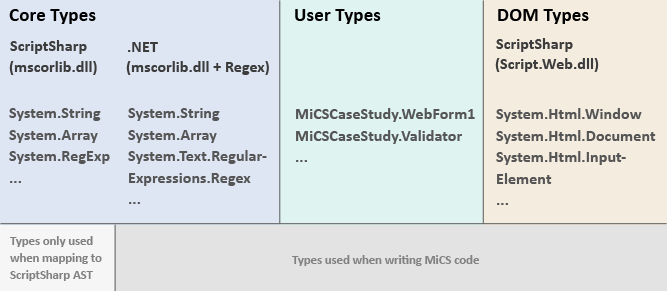
\includegraphics[width=16cm]{resources/images/TypesOverview.png}}
		\end{center}
		\caption{The different types used by MiCS.}
		\label{typesOverview}
	\end{figure}

	Since one of the goals of MiCS is to be able to execute the same code on both client and server side (server client portability) its required that the .NET core types are used when writing MiCS code. This is in contrast to how Script\# works in its original manner where the Script\# core types (that reflect the equivalent JavaScript types) are used. This has some benefits but is also an obstacle that prevents server client portability.

	\subsection{Core Types} % (fold)
	\label{sub:core_types}
		To build the ScriptSharp AST correctly the ScriptSharp core types are required to be associated to the AST nodes. One reason the ScriptSharp core types are required is that they define their equivalent script name (in the class attributes) that is used by the ScriptSharp script generator. An example is the System.Char (see figure \ref{char}) type which is converted to the JavaScript String type as no JavaScript Char type exists.

	\begin{figure}[H]
			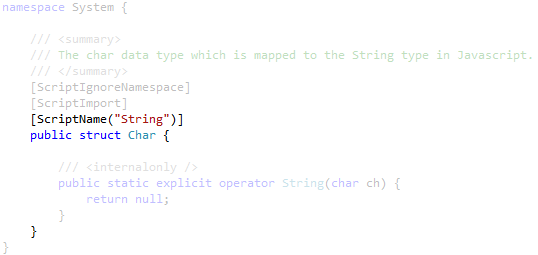
\includegraphics[width=13cm]{resources/images/Char.png}
		\caption{The core type System.Char defined in the Script\# mscorlib.dll.}
		\label{char}
	\end{figure}

		MiCS uses the regular .NET core types when a developer is writing MiCS code but when generating the client side script the Script\# defined core types are used. This implies that some kind of mapping between the two kinds of core types are required. This mapping of core types is explained in section \ref{sub:type_mapping}.
	% subsection core_types (end)

	\subsection{User Types} % (fold)
	\label{sub:user_types}
		User types are the types that are defined by the developer. The user types considered here are either MixedSide types or ClientSide types (i.e. types that have method members that have the either the MixedSide attribute or the ClientSide attribute on them). User type definitions is what the generated client side script eventually will consist of. 

		Pure server side types are obviously also user types but they are not relevant in a MiCS context as JavaScript will not be generated from them.
	% subsection user_types (end)

	\subsection{DOM Types} % (fold)
	\label{sub:dom_types}
		Document Object Model (DOM) types are Script\# infrastructure defined in the System.Html namespace (Script.Web.dll). These classes that represent DOM objects from the browser. The purpose of these classes is only to represent the interface of the actual DOM types in the browser. This is also seen if one looks at the implementation of these types as all their methods and properties on these types return null or false. Like the Script\# core types, DOM types also has their script names in the attribute [ScriptName]. The DOM types are only meant for ClientSide code.

		\begin{figure}[H]
				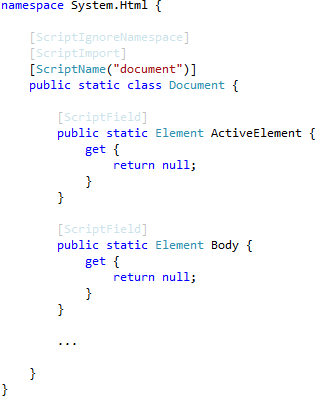
\includegraphics[width=7cm]{resources/images/Document.png}
			\caption{Script\# definition of the DOM type Document.}
			\label{fig:document}
		\end{figure}
	% subsection dom_types (end)

% section types_in_mics (end)

	\section{The MixedSide Principle} % (fold)
	\label{sub:the_mixedside_principle}
		The Mixed Side Principle is a fundamental constraint that the developer has to comply with when using MiCS. In a MiCS web application project there are three kinds of code the user can write; server side code, mixed side code (annotated with the \texttt{MixedSide attribute}) and client side code (annotated with the \texttt{ClientSide} attribute). The Mixed Side Principle describes a simple rule set for the interactions between the different kinds of code. 

		The Mixed Side Principle states that; \emph{Mixed side code can only use other mixed side code. Server and client side code can use mixed side code and code of their own kind respectively.}

		The Mixed Side Principle is illustrated in Figure \ref{fig:MixedSidePrinciple}.

		\begin{figure}[H]
			\begin{center}
				\centerline{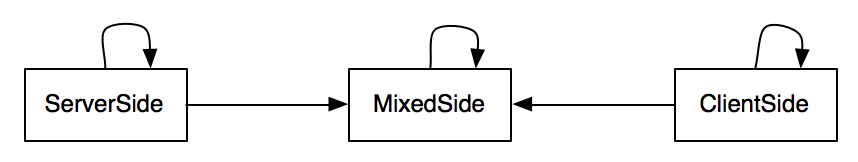
\includegraphics[width=12cm]{resources/images/MixedSidePrinciple.png}}
			\end{center}
			\caption{The Mixed Side Principle. Arrows indicate which kind of code is allowed to be used by the specific kind.}
			\label{fig:MixedSidePrinciple}
		\end{figure}

		Code annotated with the \texttt{ClientSide} attribute is only meant to be run on client side in form of generated JavaScript. Therefore client side code cannot make calls to server side only objects. This would not make sense as server and client side are two different and separated execution contexts.  If client side code were to call server side code, it would ultimately result in a client side error as the server side code will not be mapped to client side. Likewise it will not make sense for server side code to call client side code.

		However mixed side code can be called both from client and server side code. Mixed side code can however only consist of C\# constructs, supported by MiCS, that can be mapped to JavaScript. Mixed side code can only call other mixed side code therefore it cannot use client side only types such as DOM types. This would simply not make sense when mixed side code is called from server side.

		All three kinds of code can obviously use other code of the same kind hence the recursive arrows in illustartion \ref{fig:MixedSidePrinciple}.

\section{Workflow Overview} % (fold)
\label{sec:workflow_overview}

This section provides a brief overview of how MiCS works. Figure \ref{fig:mics_internal_workflow} shows the five stages that MiCS goes through when converting C\# to JavaScript.

Basically, MiCS uses Roslyn to generate an AST representing the user’s C\# code. This AST is validated and mapped to a Script\# AST, that represents JavaScript. From the Script\# AST, JavaScript is generated and finally injected into the user’s WebForm page.

\begin{figure}[H]
	\begin{center}
		\centerline{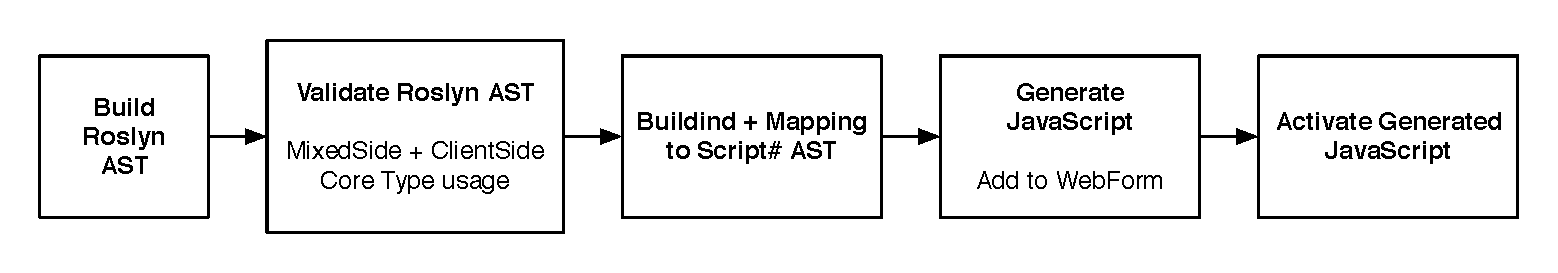
\includegraphics[width=14cm]{resources/images/internalworkflow.eps}}
	\end{center}
	\caption{The MiCS internal workflow}
	\label{fig:mics_internal_workflow}
\end{figure}

MiCS uses Roslyn to generate an Abstract Syntax Tree which is a syntatic representation of the user’s C\# code. Apart from the AST, a Semantic Model is generated to obtain information about what is being referenced.

When the Roslyn AST has been obtained it needs to be validated. This is done to ensure that the user uses types in a correct manner. Without validation, it would be possible for the user to generate non-working JavaScript.

Once the syntax tree has been validated, it is ready to be mapped to Script\#. This is the core functionality of MiCS - transforming a Roslyn AST to a Script\# AST. This step also ensures that the user does not utilize C\# constructs (declarations, statements and expressions) that we do not support. For example, at the moment the only supported loop-type is the for-loop. So if the user uses a while-loop or a foreach loop, the user gets an error telling them that an unsupported construct has been used.

When the Roslyn AST has successfully been mapped to Script\#, MiCS uses Script\#’s built-in ScriptGenerator to generate the JavaScript corresponding to the user’s original C\# code. 

When the JavaScript has been generated, it needs to be injected into the users WebForm. This is handled by a MiCSPage class; an extension to a WebForm Page. 

% section workflow_overview (end)

\section{Architecture} % (fold)
\label{sec:architecture}
Figure \ref{fig:dependencygraph} shows the most essential parts of the internal MiCS architecture and how the parts depend on each other. 
This section will describe the different parts, how they relate to one another and how the architecture relates to the five stages outlined in section \ref{sec:workflow_overview}. 

\begin{figure}
	\begin{center}
		\centerline{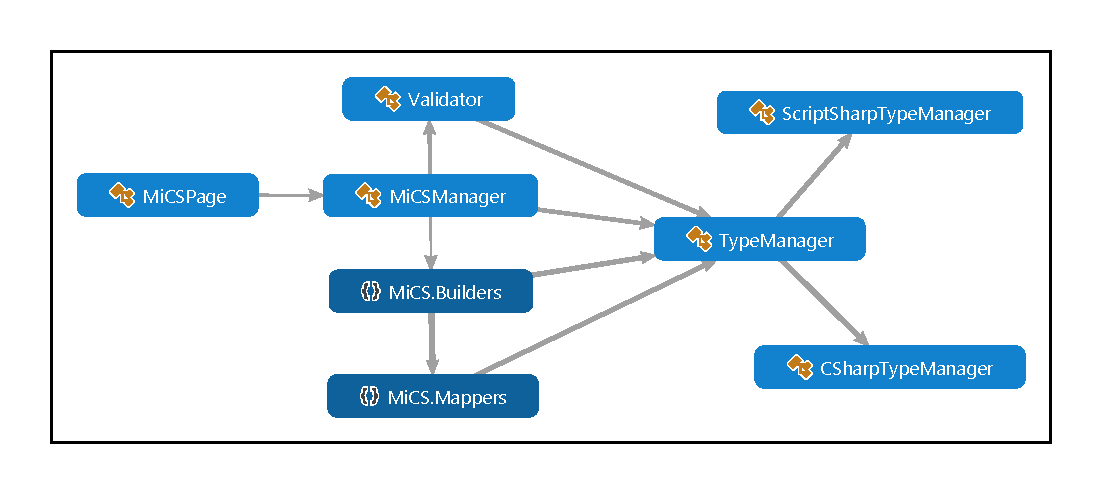
\includegraphics[width=15cm]{resources/images/architecture.pdf}}
	\end{center}
	\caption{The most important parts of the MiCS architecture.}
	\label{fig:dependencygraph}
\end{figure}


The TypeManagers (\texttt{TypeManager}, \texttt{CSharpTypeManager} and\newline \texttt{ScriptSharpTypeManager}) provide information about types used throughout MiCS. For example, the TypeManagers are able to lookup the resultant type of an expression or the type of an identifier (using the Semantic Model described in section \ref{sub:microsoft_roslyn}). Furthermore, they can determine whether a given type is one that the user has defined, or if it is a built-in .NET-type.

The \texttt{Validator} class is responsible for validating the user's code in order to ensure correct type usage before the conversion to Script\# AST begins. The \texttt{Validator} is initiated by the MiCSManager and is dependent on the type managers.

Classes in the Builders and Mappers namespaces are responsible for converting a Roslyn AST to its' corresponding Script\# AST. The Builders traverse the Roslyn AST and build a corresponding Script\# AST. The Builders are dependent on the Mappers which handle the actual conversion from Roslyn SyntaxNodes (AST nodes) to the corresponding Script\# constructs. (Stage 3)

The \texttt{MiCSManager} class ties the entire MiCS project together and is involved in all of the stages described in section \ref{sec:workflow_overview}. It initializes the TypeManagers, starts the validation, and subsequently initiates all of the processes needed to generate JavaScript. 

TODO: Vis og beskriv hvilken del af ScriptSharp vi erstatter med MiCS og Roslyn.
TODO: Update dependency graph

% % section architecture (end)

\section{Usability Considerations}
This section focuses on design considerations conserning usability for the developer. The design considerations mentioned here are mainly nice-to-haves and will not be discussed in the implementation chapter. However, we will reflect upon these considerations in the evaluation.

\subsection{What to generate JavaScript from?} % (fold)
\label{sub:what_to_generate_javascript_from}
	To easily distinguish client side code, mixed side code and server side code from one another, the \texttt{MixedSide} and \texttt{ClientSide} attributes have been introduced. They serve as an easy way for the developer to express which methods that should be used on client side, server side and mixed side respectively. At the same time, they make it easy for MiCS to understand which parts of the developers code to generate JavaScript from. The attributes needs to be used explicit to help ensure that only code intended for client side is actually generated as JavaScript.

% subsection what_to_generate_javascript_from (end)

\subsection{Error messages} % (fold)
\label{sub:design_error_messages}
	As stated in the introduction, it is not our intent to make a complete mapping from C\# to JavaScript. Therefore, when developers use a C\# construct or type that we are unable to map, it is important to fail with an error message that makes sense to the developer. It should not be left to the developer to interpret and debug errors thrown directly from Roslyn. For this reason, different exceptions are implemented. An example of such an exception is the \texttt{MixedSidePrincipleViolatedException} which is thrown, e.g. when code annotated with the \texttt{MixedSide} attribute calls either client or server side code.

	% subsection error_messages (end)

\subsection{Initializing MiCS} % (fold)
\label{sub:initializng_mics}
	There should not be a huge overhead on developers when they want to use MiCS in their projects. In order to acheive this, the process of initializing MiCS has been implemented in the \texttt{MiCSPage} class. When using MiCS, as explained in the user manual (chapter \ref{chap:mics_manual}), the \texttt{MiCSPage} class should be used instead of ASP.NET's \texttt{System.Web.UI.Page} class.
% subsection initializng_mics (end)

\section{Chapter Summary} % (fold)
\label{sec:chapter_design_summary}
In this chapter we have described the different kinds of types used in MiCS, established the Mixed Side Principle, described the overall workflow of MiCS and described how written code is annotated with attributes to indicate whether it is client or server side code. In the next chapter, the implementation of MiCS is described.
% section chapter_summary (end)